\chapter{Moteurs et machines thermiques}\label{ch:b1:heat-engines}

Un moteur de voiture, une centrale électrique, un \omterm{def:b1:heat-engines:machine}{réfrigérateur} et une
\omterm{def:b1:heat-engines:machine}{pompe à chaleur} sont un même objet vu de quatre côtés~: un fluide que l'on
fait décrire un cycle, en contact tour à tour avec une source chaude et une
source froide, échangeant de la chaleur avec les deux et du travail avec un
arbre. Le premier principe tient la comptabilité de l'énergie~; le second,
par le bilan d'entropie sur un cycle, fixe la limite qu'aucune ingéniosité
ne franchira --- le théorème de Carnot, l'inégalité la plus lourde de
conséquences de toute l'ingénierie. Ce chapitre établit cette limite,
calcule le cycle idéal et les cycles réels qui s'en approchent (Otto,
Diesel, Stirling), retourne la machine pour produire du froid et chauffer
les maisons, et montre comment l'entropie créée par une machine réelle se
paie, joule par joule, en \omterm{thm:b1:heat-engines:lostwork}{travail perdu}.

\section{Machines cycliques et les deux principes}

\begin{definition}[Machine thermodynamique]\label{def:b1:heat-engines:machine}
\index{moteur thermique}\index{réfrigérateur}\index{pompe à chaleur}\index{thermostat}
Une \emph{machine thermodynamique} est un \omterm{def:b1:newton-dynamics:conservation}{système fermé} (le fluide) que
l'on fait décrire un \emph{cycle}, de sorte qu'il revient périodiquement au
même état, tout en échangeant un travail $W$ avec l'extérieur et des
chaleurs $Q_i$ avec des sources aux températures $T_i$ --- des
\emph{thermostats}, dont l'échange ne modifie pas la température. Une
machine \emph{ditherme} utilise deux thermostats~: la source chaude à
$T_h$ et la source froide à $T_c < T_h$. C'est un \emph{moteur} si elle
fournit du travail ($W < 0$), un \emph{réfrigérateur} si elle est entraînée
($W > 0$) pour prélever de la chaleur à la source froide, une \emph{pompe
à chaleur} si elle est entraînée pour en céder à la source chaude. Toutes
les grandeurs sont comptées sur un cycle, algébriquement, comme reçues par le fluide.
\end{definition}

\begin{theorem}[Les deux principes sur un cycle~; inégalité de Clausius]\label{thm:b1:heat-engines:clausius}
\index{inégalité de Clausius}
Sur un cycle d'une machine ditherme,
\[
W + Q_h + Q_c = 0 , \qquad
\frac{Q_h}{T_h} + \frac{Q_c}{T_c} = -S_{\text{créée}} \leq 0 ,
\]
avec égalité dans la seconde relation si et seulement si le cycle est
réversible. Plus généralement, pour un nombre quelconque de \omterm{def:b1:heat-engines:machine}{thermostats},
$\sum_i Q_i/T_i \leq 0$ (\emph{inégalité de Clausius}).
\end{theorem}

\begin{proof}
$U$ et $S$ sont des fonctions d'état, donc $\Delta U = 0$ et $\Delta S = 0$ sur
un cycle. Le premier principe donne $0 = W + Q_h + Q_c$~; le bilan d'entropie
(\cref{thm:b1:second-law-entropy:secondlaw}) donne $0 = S_{\text{éch}} +
S_{\text{créée}}$ avec $S_{\text{éch}} = \sum Q_i/T_i$, chaque
\omterm{def:b1:heat-engines:machine}{thermostat} échangeant à sa propre température fixée
(\cref{prop:b1:second-law-entropy:thermostat}).
\end{proof}

\begin{corollary}[Kelvin, à nouveau]\label{cor:b1:heat-engines:kelvin}
Une machine \emph{monotherme} ($Q_c = 0$) a $Q_h \leq 0$, donc $W \geq 0$~:
aucun cycle ne peut convertir en travail la chaleur d'une source unique. Un
navire ne peut avancer en refroidissant la mer --- un moteur a besoin d'une
source froide où rejeter de la chaleur, et le second principe dit combien.
\end{corollary}

\begin{omfigure}
\begin{tikzpicture}[font=\small, x=1cm, y=1cm, >=Stealth]
  % engine
  \begin{scope}
    \draw[fill=omThm!15, draw=omThm, thick] (-1.6,3.0) rectangle (1.6,3.7) node[midway] {source chaude $T_h$};
    \draw[fill=omDef!15, draw=omDef, thick] (-1.6,-0.7) rectangle (1.6,0) node[midway] {source froide $T_c$};
    \draw[thick, rounded corners, fill=omProp!10] (-0.9,1.0) rectangle (0.9,2.0) node[midway] {moteur};
    \draw[->, omThm, very thick] (0,3.0) -- (0,2.0) node[midway, right] {$Q_h > 0$};
    \draw[->, omDef, very thick] (0,1.0) -- (0,0) node[midway, right] {$Q_c < 0$};
    \draw[->, omProp, very thick] (0.9,1.5) -- (2.3,1.5) node[midway, above] {$W < 0$};
    \node[font=\footnotesize] at (0,-1.1) {$\eta = -W/Q_h$};
  \end{scope}
  % refrigerator / heat pump
  \begin{scope}[xshift=6.4cm]
    \draw[fill=omThm!15, draw=omThm, thick] (-1.6,3.0) rectangle (1.6,3.7) node[midway] {source chaude $T_h$};
    \draw[fill=omDef!15, draw=omDef, thick] (-1.6,-0.7) rectangle (1.6,0) node[midway] {source froide $T_c$};
    \draw[thick, rounded corners, fill=omProp!10] (-1.1,1.0) rectangle (1.1,2.0) node[midway, align=center, font=\footnotesize] {réfrigérateur\\ ou pompe à chaleur};
    \draw[->, omThm, very thick] (0,2.0) -- (0,3.0) node[midway, right] {$Q_h < 0$};
    \draw[->, omDef, very thick] (0,0) -- (0,1.0) node[midway, right] {$Q_c > 0$};
    \draw[->, omProp, very thick] (-2.5,1.5) -- (-1.1,1.5) node[midway, above] {$W > 0$};
    \node[font=\footnotesize] at (0,-1.1) {$e_f = Q_c/W$, \quad $e_p = -Q_h/W$};
  \end{scope}
\end{tikzpicture}

{\small Les deux sens de parcours d'un cycle ditherme. À gauche~: le moteur
prend de la chaleur à la source chaude, en rejette une partie à la source
froide et fournit la différence en travail. À droite~: la même machine
entraînée à l'envers pompe la chaleur du froid vers le chaud~; c'est un
\omterm{def:b1:heat-engines:machine}{réfrigérateur} si l'on veut $Q_c$, une \omterm{def:b1:heat-engines:machine}{pompe à chaleur} si l'on veut $|Q_h|$.}
\end{omfigure}

\section{Le théorème de Carnot}

\begin{definition}[Rendement et efficacités]\label{def:b1:heat-engines:efficiency}
\index{rendement!d'un moteur thermique}\index{efficacité}
Le \emph{rendement} d'un moteur est le travail fourni par unité de chaleur
prélevée à la source chaude, $\eta = -W/Q_h$~; l'\emph{efficacité} d'un
\omterm{def:b1:heat-engines:machine}{réfrigérateur} est le froid produit par unité de travail, $e_f = Q_c/W$~;
celle d'une \omterm{def:b1:heat-engines:machine}{pompe à chaleur} est la chaleur fournie par unité de travail,
$e_p = -Q_h/W$. Chacun est le rapport de «~ce que l'on veut~» sur «~ce que
l'on paie~»~; un rendement vaut au plus~1, une efficacité peut dépasser~1.
\end{definition}

\begin{theorem}[Carnot]\label{thm:b1:heat-engines:carnot}
\index{théorème de Carnot}\index{rendement de Carnot}
Entre des \omterm{def:b1:heat-engines:machine}{thermostats} $T_h > T_c$,
\[
\eta \leq \eta_C = 1 - \frac{T_c}{T_h}, \qquad
e_f \leq \frac{T_c}{T_h - T_c}, \qquad
e_p \leq \frac{T_h}{T_h - T_c} = 1 + \frac{T_c}{T_h - T_c},
\]
avec égalité si et seulement si le cycle est réversible. Ces bornes ne
dépendent que des températures --- ni du fluide, ni du mécanisme.
\end{theorem}

\begin{proof}
Pour un moteur ($Q_h > 0$)~: $\eta = -W/Q_h = (Q_h + Q_c)/Q_h = 1 + Q_c/Q_h$,
et l'inégalité de Clausius donne $Q_c/Q_h \leq -T_c/T_h$. Pour un
\omterm{def:b1:heat-engines:machine}{réfrigérateur} ($Q_c > 0$, $W > 0$)~: $W = -Q_h - Q_c$ avec $-Q_h \geq Q_c T_h/T_c$,
donc $W \geq Q_c(T_h/T_c - 1)$ et $e_f = Q_c/W \leq T_c/(T_h - T_c)$.
Pour la \omterm{def:b1:heat-engines:machine}{pompe à chaleur}, $e_p = -Q_h/W = (W + Q_c)/W = 1 + e_f$. L'égalité
est le cas réversible, $S_{\text{créée}} = 0$ tout du long.
\end{proof}

\begin{example}[Trois nombres]\label{ex:b1:heat-engines:numbers}
Une turbine à vapeur entre $T_h = \qty{800}{K}$ et une rivière à
$T_c = \qty{300}{K}$~: $\eta_C = 0.625$~; les centrales réelles atteignent environ $0.40$.
Un \omterm{def:b1:heat-engines:machine}{réfrigérateur} domestique entre $\qty{275}{K}$ à l'intérieur et une cuisine à
$\qty{298}{K}$~: $e_f \leq 275/23 = 12$~; les machines réelles donnent $2$ à $4$.
Une \omterm{def:b1:heat-engines:machine}{pompe à chaleur} qui chauffe une maison à $\qty{293}{K}$ à partir d'un air à $\qty{273}{K}$~:
$e_p \leq 293/20 = 14.7$~; les pompes réelles donnent $3$ à $5$ --- trois à
cinq fois encore ce que la même électricité donnerait dans une résistance
(\cref{pb:b1:heat-engines:1}).
\end{example}

\begin{remark}[Pourquoi le rendement ne peut valoir~1]\label{rem:b1:heat-engines:why}
Un moteur reçoit l'entropie $Q_h/T_h$ avec la chaleur qu'il prélève~; le
travail n'en emporte aucune~; la seule sortie est la chaleur rejetée à la
source froide, qui en emporte $|Q_c|/T_c$. L'entropie ne pouvant être
détruite, il faut jeter au moins $Q_h T_c/T_h$ de chaleur, et le travail est
ce qui reste. Plus la source froide est basse et la source chaude haute,
mieux c'est --- d'où les tours de refroidissement, et la course aux aubes de
turbine toujours plus chaudes.
\end{remark}

\section{Le cycle de Carnot}

\begin{definition}[Cycle de Carnot]\label{def:b1:heat-engines:carnotcycle}
\index{cycle de Carnot}
Le \emph{cycle de Carnot} est le cycle ditherme réversible~: deux isothermes
réversibles, à $T_h$ (au contact de la source chaude) et à $T_c$ (au contact
de la source froide), reliées par deux adiabatiques réversibles
(isentropiques, sans contact avec aucune source). Parcouru dans le sens
horaire dans le plan $(V, P)$, c'est un moteur~; dans l'autre sens, un
\omterm{def:b1:heat-engines:machine}{réfrigérateur} ou une \omterm{def:b1:heat-engines:machine}{pompe à chaleur}. Dans le \omterm{def:b1:second-law-entropy:TS}{diagramme entropique}, c'est un rectangle.
\end{definition}

\begin{proposition}[Cycle de Carnot d'un gaz parfait]\label{prop:b1:heat-engines:carnotgas}
Pour $n$ \omterm{def:b1:kinetic-theory:scales}{moles} de \omterm{def:b1:kinetic-theory:model}{gaz parfait} décrivant $A \to B$ (isotherme $T_h$,
détente), $B \to C$ (adiabatique), $C \to D$ (isotherme $T_c$,
compression), $D \to A$ (adiabatique)~:
\[
Q_h = nRT_h\ln\frac{V_B}{V_A}, \qquad
Q_c = -nRT_c\ln\frac{V_B}{V_A}, \qquad
\eta = 1 - \frac{T_c}{T_h} ,
\]
la valeur de Carnot --- comme il se doit pour tout cycle ditherme réversible.
\end{proposition}

\begin{proof}
Sur une isotherme $\Delta U = 0$, donc $Q = -W = nRT\ln(V_{\text{final}}/
V_{\text{initial}})$. Sur les adiabatiques, $TV^{\gamma-1}$ est constant~:
$T_hV_B^{\gamma-1} = T_cV_C^{\gamma-1}$ et $T_hV_A^{\gamma-1} =
T_cV_D^{\gamma-1}$, d'où $V_C/V_D = V_B/V_A$ et $Q_c = nRT_c\ln(V_D/V_C) =
-nRT_c\ln(V_B/V_A)$. Puis $\eta = 1 + Q_c/Q_h = 1 - T_c/T_h$.
\end{proof}

\begin{omfigure}
\begin{tikzpicture}
\begin{axis}[omaxis, axis x line=bottom, axis y line=left, width=7.6cm, height=5.6cm,
    xlabel={$V$}, ylabel={$P$}, xmin=0, xmax=6.3, ymin=0, ymax=1.7,
    xlabel style={at={(axis description cs:0.5,-0.06)}, anchor=north},
    xtick=\empty, ytick=\empty, samples=60]
  \addplot[omThm, thick, domain=1:2] {1.5/x} node[pos=0.5, above right, font=\footnotesize] {$T_h$};
  \addplot[omProp, thick, domain=2:5.51] {0.75*(2/x)^1.4};
  \addplot[omDef, thick, domain=2.756:5.51] {1/x} node[pos=0.2, below left, font=\footnotesize] {$T_c$};
  \addplot[omProp, thick, domain=1:2.756] {0.3628*(2.756/x)^1.4};
  \node[font=\footnotesize, anchor=south west] at (axis cs:0.95,1.52) {$A$};
  \node[font=\footnotesize, anchor=south west] at (axis cs:2.05,0.77) {$B$};
  \node[font=\footnotesize, anchor=north west] at (axis cs:5.5,0.18) {$C$};
  \node[font=\footnotesize, anchor=north east] at (axis cs:2.7,0.35) {$D$};
  \node[font=\footnotesize, omProp] at (axis cs:4.4,0.62) {adiabatiques};
  \draw[-Stealth, thick] (axis cs:1.45,1.1) -- (axis cs:1.55,1.0);
  \draw[-Stealth, thick] (axis cs:4.3,0.22) -- (axis cs:4.1,0.235);
\end{axis}
\end{tikzpicture}\hfill
\begin{tikzpicture}
\begin{axis}[omaxis, axis x line=bottom, axis y line=left, width=6.2cm, height=5.6cm,
    xlabel={$S$}, ylabel={$T$}, xmin=-1.2, xmax=4.6, ymin=0, ymax=2.2, clip=false,
    xlabel style={at={(axis description cs:0.5,-0.1)}, anchor=north},
    xtick={1,3}, xticklabels={$S_1$,$S_2$}, ytick={0.8,1.6}, yticklabels={$T_c$,$T_h$}]
  \fill[omProp!20] (axis cs:1,0.8) rectangle (axis cs:3,1.6);
  \draw[omThm, thick, -Stealth] (axis cs:1,1.6) -- (axis cs:3,1.6) node[midway, above, font=\footnotesize] {$A \to B$};
  \draw[omProp, thick, -Stealth] (axis cs:3,1.6) -- (axis cs:3,0.8) node[midway, right, font=\footnotesize] {$B \to C$};
  \draw[omDef, thick, -Stealth] (axis cs:3,0.8) -- (axis cs:1,0.8) node[midway, below, font=\footnotesize] {$C \to D$};
  \draw[omProp, thick, -Stealth] (axis cs:1,0.8) -- (axis cs:1,1.6) node[midway, left, font=\footnotesize] {$D \to A$};
  \node[font=\footnotesize] at (axis cs:2,1.2) {$-W$};
\end{axis}
\end{tikzpicture}

{\small Le \omterm{def:b1:heat-engines:carnotcycle}{cycle de Carnot} d'un \omterm{def:b1:kinetic-theory:model}{gaz parfait}. À gauche~: dans le diagramme
de Clapeyron, deux isothermes et deux adiabatiques (plus raides), parcourues
dans le sens horaire~; l'aire enclose est le travail fourni. À droite~: le
même cycle dans le \omterm{def:b1:second-law-entropy:TS}{diagramme entropique} est un rectangle de hauteur
$T_h - T_c$ et de largeur $Q_h/T_h$~; son aire vaut encore $-W$, et le rapport
de cette aire à celle sous le côté supérieur, $Q_h$, vaut $1 - T_c/T_h$ à vue.}
\end{omfigure}

\begin{remark}[Le cycle de Carnot est un théorème, pas un moteur]\label{rem:b1:heat-engines:notengine}
Des isothermes réversibles exigent un transfert thermique infiniment lent
sous un écart de température qui tend vers zéro~: un moteur de Carnot
fournit son travail maximal à puissance nulle. Les machines réelles
échangent du \omterm{def:b1:heat-engines:efficiency}{rendement} contre de la puissance en acceptant des écarts de
température finis dans leurs échangeurs
(\cref{exo:b1:heat-engines:10})~; la valeur de Carnot reste le plafond
auquel se mesure toute conception.
\end{remark}

\section{Les cycles moteurs réels}

\begin{proposition}[Cycle Otto]\label{prop:b1:heat-engines:otto}
\index{cycle Otto}\index{taux de compression}
Le moteur à essence idéalisé fait décrire à l'air ($\gamma$)~: $1 \to 2$
compression adiabatique de $V_1$ à $V_2$ (\emph{\omterm{prop:b1:heat-engines:otto}{taux de compression}}
$r = V_1/V_2$)~; $2 \to 3$ échauffement isochore (la combustion)~; $3 \to 4$
détente adiabatique jusqu'à $V_1$~; $4 \to 1$ refroidissement isochore
(l'échappement). Son \omterm{def:b1:heat-engines:efficiency}{rendement} vaut
\[
\eta_{\text{Otto}} = 1 - \frac{1}{r^{\gamma-1}} .
\]
\end{proposition}

\begin{proof}
La chaleur n'est échangée que sur les isochores~: $Q_h = nC_{V,m}(T_3 - T_2)$ et
$Q_c = nC_{V,m}(T_1 - T_4)$. Sur les adiabatiques, $TV^{\gamma-1}$ est constant~:
$T_2 = T_1r^{\gamma-1}$ et $T_3 = T_4r^{\gamma-1}$, donc $T_3 - T_2 =
(T_4 - T_1)r^{\gamma-1}$ et
$\eta = 1 + Q_c/Q_h = 1 - (T_4 - T_1)/(T_3 - T_2) = 1 - r^{1-\gamma}$.
\end{proof}

\begin{example}[Nombres pour un moteur à essence]\label{ex:b1:heat-engines:ottonumbers}
$r = 9$, $\gamma = 1.4$~: $9^{0.4} = 2.41$ et $\eta = 0.58$. Un moteur réel
donne environ $0.30$~: la combustion n'est pas instantanée, le gaz n'est pas
parfait à \qty{2500}{K}, la chaleur fuit aux parois, le frottement et le
pompage prennent leur part. Augmenter $r$ aide --- jusqu'à ce que le mélange
air--carburant s'enflamme de lui-même en fin de compression (le cliquetis)~;
le moteur Diesel fait de ce vice son principe.
\end{example}

\begin{proposition}[Cycle Diesel]\label{prop:b1:heat-engines:diesel}
\index{cycle Diesel}
Remplaçons l'échauffement isochore du \omterm{prop:b1:heat-engines:otto}{cycle Otto} par un échauffement isobare,
de $V_2$ à $V_3 = \rho V_2$ (\emph{taux d'injection} $\rho > 1$)~: le carburant,
injecté dans un air déjà chaud d'un \omterm{prop:b1:heat-engines:otto}{taux de compression} $r$ de $15$ à $22$,
brûle à mesure qu'il arrive. Alors
\[
\eta_{\text{Diesel}} = 1 - \frac{1}{r^{\gamma-1}}\,\frac{\rho^{\gamma} - 1}{\gamma(\rho - 1)} ,
\]
plus petit que la valeur Otto pour le même $r$, mais atteint avec des $r$
bien plus grands, donc plus grand en pratique ($0.40$ à $0.45$ pour les gros moteurs).
\end{proposition}

\begin{proof}
$Q_h = nC_{P,m}(T_3 - T_2)$, $Q_c = nC_{V,m}(T_1 - T_4)$, donc $\eta = 1 -
(T_4 - T_1)/[\gamma(T_3 - T_2)]$. Avec $T_2 = T_1r^{\gamma-1}$, $T_3 =
\rho T_2$ et, sur l'adiabatique $3 \to 4$ ($V_4 = V_1 = rV_2$), $T_4 =
T_3(V_3/V_4)^{\gamma-1} = \rho T_1 r^{\gamma-1}(\rho/r)^{\gamma-1} = T_1\rho^{\gamma}$~:
$\eta = 1 - (\rho^\gamma - 1)/[\gamma r^{\gamma-1}(\rho - 1)]$.
\end{proof}

\begin{omfigure}
\begin{tikzpicture}
\begin{axis}[omaxis, axis x line=bottom, axis y line=left, width=7.2cm, height=5.6cm,
    xlabel={$V$}, ylabel={$P$}, xmin=0, xmax=5.6, ymin=0, ymax=15.5, clip=false,
    xlabel style={at={(axis description cs:0.5,-0.06)}, anchor=north},
    xtick={1,4}, xticklabels={$V_2$,$V_1$}, ytick=\empty, samples=60]
  \addplot[omProp, thick, domain=1:4] {x^(-1.4)*6.96};
  \addplot[omThm, very thick] coordinates {(1,6.96) (1,13.9)};
  \addplot[omProp, thick, domain=1:4] {13.9*x^(-1.4)};
  \addplot[omDef, very thick] coordinates {(4,2.0) (4,1)};
  \node[font=\footnotesize, anchor=north east] at (axis cs:3.95,0.95) {$1$};
  \node[font=\footnotesize, anchor=east] at (axis cs:0.9,6.96) {$2$};
  \node[font=\footnotesize, anchor=south west] at (axis cs:1.05,13.9) {$3$};
  \node[font=\footnotesize, anchor=south west] at (axis cs:4.05,2.1) {$4$};
  \node[font=\footnotesize, omThm, anchor=west] at (axis cs:1.15,10.5) {$Q_h$ (combustion)};
  \node[font=\footnotesize, omDef, anchor=west] at (axis cs:4.15,1.0) {$Q_c$ (échappement)};
  \draw[-Stealth, thick] (axis cs:2.0,5.25) -- (axis cs:2.2,4.6);
  \draw[-Stealth, thick] (axis cs:2.2,2.33) -- (axis cs:2.0,2.65);
  \node[font=\footnotesize, omProp, anchor=west] (lblexp) at (axis cs:2.9,6.4) {détente};
  \draw[omProp, -Stealth] (lblexp.west) -- (axis cs:2.55,3.9);
  \node[font=\footnotesize, omProp, anchor=west] (lblcomp) at (axis cs:4.4,4.6) {compression};
  \draw[omProp, -Stealth] (lblcomp.west) -- (axis cs:3.3,1.45);
\end{axis}
\end{tikzpicture}\hfill
\begin{tikzpicture}
\begin{axis}[omaxis, axis x line=bottom, axis y line=left, width=6.6cm, height=5.6cm,
    xlabel={$r$}, ylabel={$\eta$}, xmin=0, xmax=22, ymin=0, ymax=1.05,
    xlabel style={at={(axis description cs:0.5,-0.12)}, anchor=north},
    xtick={5,10,15,20}, ytick={0.2,0.4,0.6,0.8,1}, samples=80]
  \addplot[omThm, thick, domain=1:22] {1-x^(-0.4)} node[pos=0.55, above, font=\footnotesize] {Otto, $\gamma = 1.4$};
  \addplot[omDef, thick, domain=1.5:22] {1-(2^1.4-1)/(1.4*x^0.4*(2-1))} node[pos=0.415, below right, font=\footnotesize, align=left] {Diesel,\\ $\rho = 2$};
  \addplot[omProp, dashed, thick] coordinates {(9,0) (9,0.585)};
  \addplot[omProp, dashed, thick] coordinates {(18,0) (18,0.632)};
\end{axis}
\end{tikzpicture}

{\small À gauche~: le \omterm{prop:b1:heat-engines:otto}{cycle Otto} dans le diagramme de Clapeyron (tracé avec $r = 4$)~:
deux adiabatiques et deux isochores~; la chaleur entre au point mort haut et
sort avec l'échappement. À droite~: \omterm{def:b1:heat-engines:efficiency}{rendements} idéaux en fonction du \omterm{prop:b1:heat-engines:otto}{taux de
compression}~; les traits pointillés marquent un moteur à essence ($r = 9$) et
un Diesel ($r = 18$, $\rho = 2$).}
\end{omfigure}

\begin{proposition}[Cycle de Stirling et régénérateur]\label{prop:b1:heat-engines:stirling}
\index{cycle de Stirling}\index{régénérateur}
Deux isothermes ($T_c$, $T_h$) reliées par deux isochores. La chaleur des
portions isochores, $\pm nC_{V,m}(T_h - T_c)$, est égale et opposée~; si elle
est stockée lors du refroidissement dans un \emph{régénérateur} (une masse
poreuse que le gaz traverse) puis restituée lors du réchauffement, seules les
isothermes échangent avec les sources, et $\eta = 1 - T_c/T_h$~: le moteur
Stirling est un moteur de Carnot à la forme de son cycle près. Sans
régénérateur, la chaleur des isochores doit venir de la source chaude et
$\eta = \dfrac{nR(T_h - T_c)\ln(V_1/V_2)}{nRT_h\ln(V_1/V_2) + nC_{V,m}(T_h - T_c)}$,
sensiblement moins (\cref{exo:b1:heat-engines:8}).
\end{proposition}

\begin{proof}
Sur les isothermes, $Q_h = nRT_h\ln(V_1/V_2)$ et $Q_c = -nRT_c\ln(V_1/V_2)$, donc
$-W = Q_h + Q_c + 0$ une fois les chaleurs isochores compensées~; on divise par
la chaleur réellement prélevée à la source chaude dans chaque cas.
\end{proof}

\begin{remark}[Turbines à vapeur et à gaz]\label{rem:b1:heat-engines:turbines}
Les centrales n'utilisent pas un gaz dans un cylindre, mais de l'eau que
l'on vaporise, détend dans une turbine, condense puis repompe (le cycle de
Rankine, avec deux changements d'état --- \cref{ch:b1:phase-changes}), ou de
l'air comprimé, chauffé par combustion et détendu dans une turbine à gaz (le
cycle de Brayton, deux adiabatiques et deux isobares). Leur analyse demande
le bilan énergétique d'un fluide en écoulement, donné dans le volume de
deuxième année~; la borne de Carnot et la logique de ce chapitre s'appliquent sans changement.
\end{remark}

\section{Réfrigérateurs et pompes à chaleur}

\begin{definition}[Cycle à compression de vapeur]\label{def:b1:heat-engines:vapourcycle}
\index{cycle à compression de vapeur}\index{fluide frigorigène}
Presque tous les \omterm{def:b1:heat-engines:machine}{réfrigérateurs}, congélateurs, climatiseurs et \omterm{def:b1:heat-engines:machine}{pompes à
chaleur} font circuler un \emph{fluide frigorigène} à travers quatre organes~:
un \emph{compresseur} (qui reçoit le travail et élève la pression de la
vapeur), un \emph{condenseur} (où la vapeur chaude se liquéfie à haute
pression en libérant $|Q_h|$ du côté chaud), un \emph{détendeur} (où le
liquide passe à basse pression sans travail ni chaleur, en se vaporisant
partiellement) et un \emph{évaporateur} (où le reste bout à basse pression en
absorbant $Q_c$ du côté froid). La chaleur est transportée en chaleur latente
de vaporisation, et les deux pressions fixent les deux températures
d'ébullition (\cref{ch:b1:phase-changes}).
\end{definition}

\begin{omfigure}
\begin{tikzpicture}[font=\small, x=1cm, y=1cm, >=Stealth, box/.style={draw, thick, rounded corners, minimum width=2.3cm, minimum height=0.8cm, align=center}]
  \node[box, fill=omThm!12] (cond) at (0,2.2) {condenseur\\ \footnotesize $P$ élevée, $T_{\mathrm{cd}}$};
  \node[box, fill=omDef!12] (evap) at (0,-2.2) {évaporateur\\ \footnotesize $P$ basse, $T_{\mathrm{ev}}$};
  \node[box, fill=omProp!12] (comp) at (3.4,0) {compresseur};
  \node[box, fill=omExo!12] (valve) at (-3.4,0) {détendeur};
  \draw[->, thick] (evap.east) -| (comp.south) node[pos=0.75, right, font=\footnotesize] {vapeur};
  \draw[->, thick] (comp.north) |- (cond.east) node[pos=0.25, right, font=\footnotesize] {vapeur chaude};
  \draw[->, thick] (cond.west) -| (valve.north) node[pos=0.75, left, font=\footnotesize] {liquide};
  \draw[->, thick] (valve.south) |- (evap.west) node[pos=0.25, left, font=\footnotesize] {liquide + vapeur};
  \draw[->, omThm, very thick] (cond.north) -- ++(0,0.8) node[above, font=\footnotesize] {$|Q_h|$ vers le côté chaud ($T_h < T_{\mathrm{cd}}$)};
  \draw[->, omDef, very thick] (0,-3.8) node[below, font=\footnotesize] {$Q_c$ pris au côté froid ($T_c > T_{\mathrm{ev}}$)} -- (evap.south);
  \draw[->, omProp, very thick] (5.6,0) node[right, font=\footnotesize] {$W$} -- (comp.east);
\end{tikzpicture}

{\small Le \omterm{def:b1:heat-engines:vapourcycle}{cycle à compression de vapeur}. Le \omterm{def:b1:heat-engines:vapourcycle}{fluide frigorigène} bout dans
l'évaporateur, plus froid que le côté froid, et se condense dans le
condenseur, plus chaud que le côté chaud~: la chaleur circule dans le sens
naturel à travers chaque échangeur, et le compresseur paie pour la faire
remonter de $T_{\mathrm{ev}}$ à $T_{\mathrm{cd}}$.}
\end{omfigure}

\begin{proposition}[Le prix des écarts de température]\label{prop:b1:heat-engines:gaps}
Une machine réversible qui travaille entre ses propres températures internes
$T_{\mathrm{ev}} < T_c$ et $T_{\mathrm{cd}} > T_h$ a $e_p = T_{\mathrm{cd}}/(T_{\mathrm{cd}} - T_{\mathrm{ev}})$,
inférieure à la valeur de Carnot entre les sources~; une machine réelle n'en
atteint qu'une fraction (typiquement $0.4$ à $0.6$). Les performances d'une
\omterm{def:b1:heat-engines:machine}{pompe à chaleur} chutent donc lorsque la température extérieure baisse et
lorsque la température exigée par le circuit de chauffage monte.
\end{proposition}

\begin{proof}
Il suffit d'appliquer le \cref{thm:b1:heat-engines:carnot} au fluide, dont
les \omterm{def:b1:heat-engines:machine}{thermostats} sont en fait les températures des échangeurs~; $T_{\mathrm{cd}} - T_{\mathrm{ev}} >
T_h - T_c$ abaisse le rapport.
\end{proof}

\begin{omfigure}
\begin{tikzpicture}
\begin{axis}[omaxis, axis x line=bottom, axis y line=left, width=10cm, height=7cm,
    xlabel={température extérieure (\unit{\degreeCelsius})}, ylabel={$e_p$},
    xlabel style={at={(axis description cs:0.5,-0.08)}, anchor=north},
    xmin=-21, xmax=16, ymin=0, ymax=16, xtick={-20,-10,0,10}, ytick={2,4,...,14}, samples=80, clip=false]
  \addplot[omThm, thick, domain=-20:1.5] {293/(20-x)};
  \node[omThm, font=\footnotesize, anchor=west] at (axis cs:-20,13.9) {Carnot, maison / air extérieur};
  \addplot[omDef, thick, domain=-20:15] {313/(321-(273+x))};
  \node[omDef, font=\footnotesize, anchor=south east] at (axis cs:15.5,10.3) {Carnot avec les écarts aux échangeurs};
  \addplot[omProp, thick, domain=-20:15] {0.55*313/(321-(273+x))};
  \node[omProp, font=\footnotesize, anchor=south west] at (axis cs:-19.5,3.1) {machine réelle};
  \addplot[black, dashed] coordinates {(-21,1) (16,1)} node[pos=0.9, above, font=\footnotesize] {résistance};
\end{axis}
\end{tikzpicture}

{\small \omterm{def:b1:heat-engines:efficiency}{Efficacité} d'une \omterm{def:b1:heat-engines:machine}{pompe à chaleur} en fonction de la température
extérieure~: la borne de Carnot entre la maison (\qty{20}{\degreeCelsius}) et
l'air extérieur~; la borne une fois comptés les écarts de température aux
échangeurs ($T_{\mathrm{cd}} = \qty{313}{K}$, $T_{\mathrm{ev}} = T_{\mathrm{ext}} - \qty{8}{K}$)~;
et une machine réaliste à $0.55$ de cette dernière. Même à \qty{-10}{\degreeCelsius}, la pompe réelle fournit environ
trois joules de chaleur par joule d'électricité, là où une résistance en
donne un.}
\end{omfigure}

\begin{example}[Pompe à chaleur ou résistance~?]\label{ex:b1:heat-engines:hpvsresistor}
Une maison qui perd \qty{6}{kW} par \qty{-5}{\degreeCelsius} au-dehors demande
\qty{6}{kW} d'électricité avec des résistances~; une \omterm{def:b1:heat-engines:machine}{pompe à chaleur} idéale
de \qty{268}{K} vers \qty{293}{K} n'en demanderait que $6/11.7 = \qty{0.51}{kW}$~;
une pompe réelle, avec des températures d'échangeurs de \qty{260}{K} et
\qty{313}{K} et un \omterm{def:b1:transient-regimes:secondorder}{facteur de qualité} $0.55$, soit $e_p = 0.55 \times 313/53 = 3.2$, en demande \qty{1.9}{kW}.
Le problème du week-end parcourt toute la saison, entropie comprise.
\end{example}

\section{Entropie et travail perdu}

\begin{theorem}[Travail perdu]\label{thm:b1:heat-engines:lostwork}
\index{travail perdu}
Un moteur ditherme qui crée l'entropie $S_{\text{créée}}$ par cycle
fournit
\[
-W = Q_h\Bigl(1 - \frac{T_c}{T_h}\Bigr) - T_c\,S_{\text{créée}} ,
\]
et une \omterm{def:b1:heat-engines:machine}{pompe à chaleur} ditherme qui fournit $|Q_h|$ consomme
$W = |Q_h|(1 - T_c/T_h) + T_c\,S_{\text{créée}}$~: chaque joule par \omterm{def:b1:kinetic-theory:temperature}{kelvin}
créé coûte $T_c$ joules de travail, la température de la source froide étant
le taux de change entre entropie et travail.
\end{theorem}

\begin{proof}
D'après le \cref{thm:b1:heat-engines:clausius}, $Q_c = -T_c(Q_h/T_h + S_{\text{créée}})$~;
on reporte dans $-W = Q_h + Q_c$. Pour la pompe, on écrit les deux mêmes
relations avec $Q_h < 0$.
\end{proof}

\begin{method}[Auditer une machine]\label{meth:b1:heat-engines:audit}
Mesurer (ou calculer) les chaleurs échangées avec chaque source ainsi que le
travail~; vérifier le premier principe~; calculer $S_{\text{créée}} = -\sum Q_i/T_i$ par cycle
ou par seconde~; la puissance perdue vaut $T_c\dot S_{\text{créée}}$~; localiser
la création (écarts de température finis dans les échangeurs, frottement,
détente à travers un robinet, compression non quasi statique) en appliquant
le bilan d'entropie à chaque organe tour à tour. Un organe qui ne crée pas
d'entropie ne vaut pas la peine d'être amélioré.
\end{method}

\begin{example}[Audit d'une centrale]\label{ex:b1:heat-engines:audit}
Source chaude \qty{800}{K}, rivière \qty{300}{K}, $\qty{1.0}{GW}$ d'électricité
à $\eta = 0.40$~: $\dot Q_h = \qty{2.5}{GW}$, $\dot Q_c = \qty{1.5}{GW}$, donc
$\dot S_{\text{créée}} = 1.5/300 - 2.5/800 = \qty{1.9}{MW/K}$ et la puissance
perdue vaut $300 \times 1.9 = \qty{0.56}{GW}$~: exactement l'écart entre la
production de Carnot $0.625 \times 2.5 = \qty{1.56}{GW}$ et le \qty{1.0}{GW} réel.
La rivière s'échauffe des \qty{1.5}{GW} qu'elle doit emporter~; l'été, quand
elle est chaude et basse, les centrales réduisent la charge.
\end{example}

\section{Exercices}

\begin{exercise}[$\star$]\label{exo:b1:heat-engines:1}
Une centrale prélève de la chaleur à \qty{800}{K} et la rejette à une rivière
à \qty{300}{K}. \omterm{thm:b1:heat-engines:carnot}{Rendement de Carnot}~; si le \omterm{def:b1:heat-engines:efficiency}{rendement} réel vaut $0.40$ et la
production électrique \qty{1.0}{GW}, chaleur prélevée au combustible et
chaleur rejetée à la rivière par seconde.
\end{exercise}

\begin{exercise}[$\star$]\label{exo:b1:heat-engines:2}
Un \omterm{def:b1:heat-engines:machine}{réfrigérateur} maintient son intérieur à \qty{275}{K} dans une cuisine à
\qty{298}{K}. \omterm{def:b1:heat-engines:efficiency}{Efficacité} maximale~; avec une \omterm{def:b1:heat-engines:efficiency}{efficacité} réelle de $3$,
\omterm{thm:b1:dc-circuits:kirchhoff}{puissance électrique} nécessaire pour évacuer les \qty{100}{W} qui entrent par
les parois.
\end{exercise}

\begin{exercise}[$\star$]\label{exo:b1:heat-engines:3}
\omterm{def:b1:heat-engines:efficiency}{Rendement} idéal d'un \omterm{prop:b1:heat-engines:otto}{cycle Otto} avec $r = 9$ et $\gamma = 1.4$~; puis avec
$r = 11$ (un moteur moderne à injection directe). Pourquoi pas $r = 20$~?
\end{exercise}

\begin{exercise}[$\star$]\label{exo:b1:heat-engines:4}
Une \omterm{def:b1:heat-engines:machine}{pompe à chaleur} chauffe une maison à \qty{300}{K} à partir d'un air
extérieur à \qty{280}{K}. $e_p$ maximale~; \omterm{thm:b1:dc-circuits:kirchhoff}{puissance électrique} pour un besoin
de chauffage de \qty{5}{kW} avec cette pompe idéale, puis avec une pompe
réelle de $e_p = 3.5$~; comparer avec une résistance.
\end{exercise}

\begin{exercise}[$\star\star$]\label{exo:b1:heat-engines:5}
Une \omterm{def:b1:kinetic-theory:scales}{mole} de \omterm{def:b1:kinetic-theory:model}{gaz parfait} ($\gamma = 1.4$) décrit un \omterm{def:b1:heat-engines:carnotcycle}{cycle de Carnot} entre
$T_h = \qty{500}{K}$ et $T_c = \qty{300}{K}$~; l'isotherme chaude la mène de
\qty{1.0}{L} à \qty{3.0}{L}. Calculer $V_C$, $V_D$, $Q_h$, $Q_c$, $W$ et
vérifier le \omterm{def:b1:heat-engines:efficiency}{rendement}.
\end{exercise}

\begin{exercise}[$\star\star$]\label{exo:b1:heat-engines:6}
Un inventeur annonce une machine cyclique qui prélève \qty{1000}{J} par cycle
à une source à \qty{400}{K}, en rejette \qty{800}{J} à une source à
\qty{300}{K} et fournit \qty{200}{J} de travail. Est-ce possible~? Entropie
créée par cycle. Un second inventeur annonce \qty{300}{J} de travail à partir
des mêmes \qty{1000}{J}, en n'en rejetant que \qty{700}{J}. Est-ce possible~?
Quel est le travail maximal que l'on puisse tirer de ces \qty{1000}{J}~?
\end{exercise}

\begin{exercise}[$\star\star$]\label{exo:b1:heat-engines:7}
\omterm{prop:b1:heat-engines:diesel}{Cycle Diesel} avec $r = 18$, $\rho = 2$, $\gamma = 1.4$~: \omterm{def:b1:heat-engines:efficiency}{rendement}~; comparer
à un \omterm{prop:b1:heat-engines:otto}{cycle Otto} de même $r$, puis au \omterm{prop:b1:heat-engines:otto}{cycle Otto} pour $r = 9$. Pourquoi le
Diesel peut-il employer un $r$ aussi grand~?
\end{exercise}

\begin{exercise}[$\star\star$]\label{exo:b1:heat-engines:8}
\omterm{prop:b1:heat-engines:stirling}{Cycle de Stirling} d'une \omterm{def:b1:kinetic-theory:scales}{mole} de \omterm{prop:b1:kinetic-theory:Ugas}{gaz diatomique} ($C_{V,m} = \tfrac52R$) entre
\qty{600}{K} et \qty{300}{K}, avec un rapport de volumes $V_1/V_2 = 2$. Travail
par cycle~; \omterm{def:b1:heat-engines:efficiency}{rendement} avec un régénérateur parfait, puis sans.
\end{exercise}

\begin{exercise}[$\star\star$]\label{exo:b1:heat-engines:9}
Deux blocs identiques de capacité thermique $C = \qty{4.0}{kJ/K}$ à $T_1 =
\qty{400}{K}$ et $T_2 = \qty{300}{K}$ servent de sources à un moteur jusqu'à ce
qu'ils atteignent une température commune $T_f$. Montrer que le travail maximal
est obtenu pour un moteur réversible, qu'alors $T_f = \sqrt{T_1T_2}$, et
calculer $W_{\max}$. Que vaudrait $T_f$ si l'on mettait simplement les blocs
en contact, et quelle entropie serait alors créée~?
\end{exercise}

\begin{exercise}[$\star\star\star$]\label{exo:b1:heat-engines:10}
\emph{Moteur à puissance maximale.} Un moteur réversible travaille entre
les températures internes $x$ et $y$, et échange de la chaleur avec les
sources à travers des échangeurs de conductance $K$~: $\dot Q_h = K(T_h - x)$ et
$|\dot Q_c| = K(y - T_c)$. (a) Écrire la puissance $P$ et la condition
d'entropie du cœur réversible. (b) Montrer que $y = xT_c/(2x - T_h)$ et
que $P = \frac{K}{2}\bigl[(T_h + T_c) - u - T_hT_c/u\bigr]$ avec $u = 2x - T_h$.
(c) Maximiser en $u$ et montrer que le \omterm{def:b1:heat-engines:efficiency}{rendement} à puissance maximale vaut
$\eta^\ast = 1 - \sqrt{T_c/T_h}$. (d) Applications numériques pour $T_h = \qty{800}{K}$,
$T_c = \qty{300}{K}$~; comparer à l'\cref{exo:b1:heat-engines:1}.
\end{exercise}

\begin{exercise}[$\star\star\star$]\label{exo:b1:heat-engines:11}
\emph{\omterm{def:b1:heat-engines:machine}{Réfrigérateur} à absorption.} Une machine sans pièce mobile prélève
la chaleur $Q_h$ à un brûleur à $T_h$, la chaleur $Q_c$ à une chambre
froide à $T_c$, et rejette de la chaleur à la pièce à $T_0$ ($T_c < T_0 <
T_h$), sans aucun travail. Montrer que
$Q_c/Q_h \leq \bigl(1 - T_0/T_h\bigr)\,T_c/(T_0 - T_c)$, interpréter les
deux facteurs, et calculer la borne pour $T_h = \qty{400}{K}$, $T_0 =
\qty{300}{K}$, $T_c = \qty{275}{K}$.
\end{exercise}

\begin{exercise}[$\star\star\star$]\label{exo:b1:heat-engines:12}
\emph{Chauffer à l'électricité, de trois façons.} L'électricité est
produite dans une centrale thermique de \omterm{def:b1:heat-engines:efficiency}{rendement} $0.40$. Par joule de
chaleur de combustible, quelle chaleur parvient à une maison (a) par une
résistance, (b) par une \omterm{def:b1:heat-engines:machine}{pompe à chaleur} de $e_p = 3.5$, (c) si le combustible
est brûlé directement dans une chaudière de \omterm{def:b1:heat-engines:efficiency}{rendement} $0.90$~? (d) L'idéal~:
un moteur réversible entre \qty{800}{K} et \qty{293}{K} entraînant une \omterm{def:b1:heat-engines:machine}{pompe
à chaleur} réversible entre \qty{273}{K} et \qty{293}{K} --- quelle chaleur par
joule de combustible, et pourquoi la réponse dépasse-t-elle un sans rien contredire~?
\end{exercise}

\begin{omfigure}
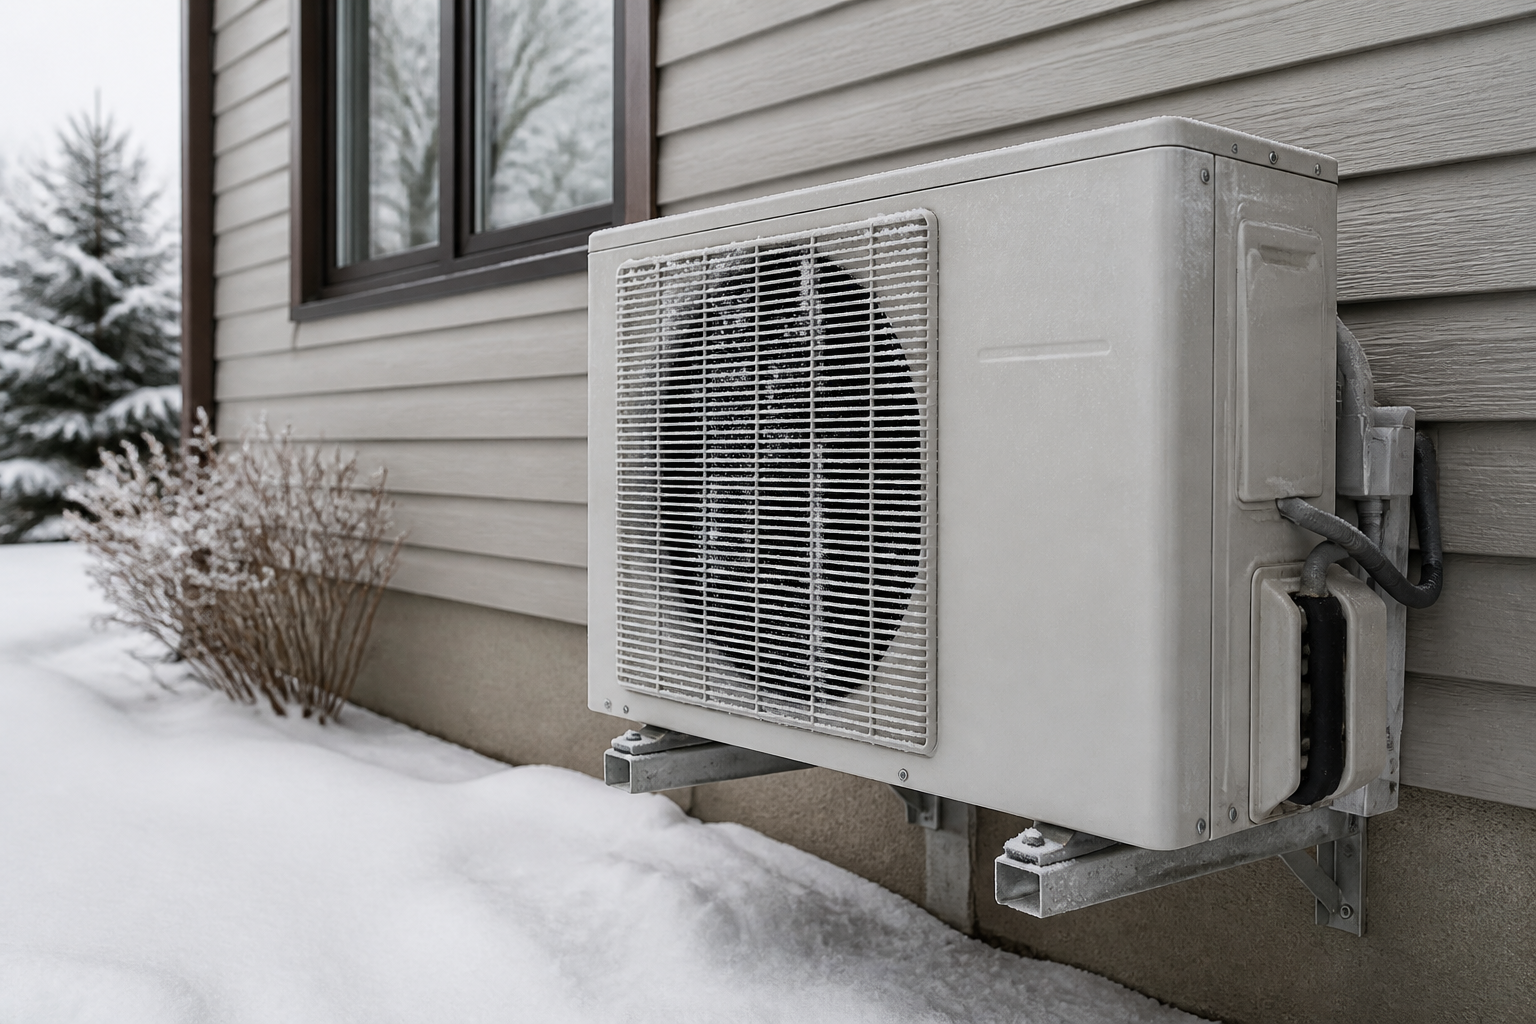
\includegraphics[width=0.58\linewidth]{images/book3/ai/b3-24-heat-pump-winter.png}

{\small Une \omterm{def:b1:heat-engines:machine}{pompe à chaleur} sur air extérieur, en hiver~: elle prélève de la chaleur à l'air froid du dehors et délivre à la maison trois à quatre fois l'énergie électrique qu'elle consomme --- c'est le problème du week-end.}
\end{omfigure}

\section{Problème~: la pompe à chaleur de la maison}

\begin{problem}[{Problème du week-end --- chauffer une maison tout un
hiver~: la facture avec des résistances, avec du gaz, avec une pompe à
chaleur idéale et avec une pompe réelle, et où passe l'électricité de cette dernière}]
\label{pb:b1:heat-engines:1}
Une maison perd de la chaleur au rythme $K(T_{\mathrm{int}} - T_{\mathrm{ext}})$ avec
$K = \qty{250}{W/K}$~; elle est maintenue à $T_{\mathrm{int}} = \qty{20}{\degreeCelsius}$.
Température extérieure de base $\qty{-5}{\degreeCelsius}$~; saison de chauffe~:
$200$ jours à une température extérieure moyenne de \qty{7}{\degreeCelsius}.
Prix~: électricité 0.25~\texteuro{} le \unit{kW h}, gaz 0.10~\texteuro{} le
\unit{kW h}~; $\qty{1}{kW h} = \qty{3.6}{MJ}$.

\medskip
\noindent\textbf{Partie I --- La maison et les procédés anciens.}
\begin{enumerate}
  \item Puissance de chauffage nécessaire à la température de base.
  \item Énergie nécessaire sur la saison, en joules et en \unit{kW h}.
  \item Coût de la saison avec des résistances électriques.
  \item Coût avec une chaudière à gaz de \omterm{def:b1:heat-engines:efficiency}{rendement} $0.90$.
  \item L'électricité vient d'une centrale thermique de \omterm{def:b1:heat-engines:efficiency}{rendement}
        $0.40$. Énergie de combustible consommée sur la saison par les
        résistances puis par la chaudière~; commenter l'idée que «~le
        chauffage électrique est thermodynamiquement dispendieux~».
\end{enumerate}

\medskip
\noindent\textbf{Partie II --- La \omterm{def:b1:heat-engines:machine}{pompe à chaleur} idéale.}
\begin{enumerate}[resume]
  \item Définir $e_p$ et démontrer, à partir des deux principes sur un
        cycle, que $e_p \leq T_{\mathrm{int}}/(T_{\mathrm{int}} - T_{\mathrm{ext}})$.
  \item $e_p$ idéale à la température de base, et \omterm{thm:b1:dc-circuits:kirchhoff}{puissance électrique}
        alors nécessaire.
  \item $e_p$ idéale à la température moyenne de la saison, et (en retenant
        cette valeur pour toute la saison) l'électricité saisonnière.
  \item Expliquer physiquement pourquoi $e_p$ diminue lorsque la température
        extérieure baisse, et pourquoi c'est le pire comportement possible
        pour un appareil de chauffage.
  \item Au point de base, la pompe idéale consomme \qty{0.53}{kW} et
        fournit \qty{6.25}{kW}~: d'où viennent les \qty{5.7}{kW} restants,
        et pourquoi refroidir l'air extérieur froid pour chauffer une
        maison chaude ne viole-t-il pas le second principe~?
\end{enumerate}

\medskip
\noindent\textbf{Partie III --- La machine réelle.}
La pompe décrit un \omterm{def:b1:heat-engines:vapourcycle}{cycle à compression de vapeur}. Le \omterm{def:b1:heat-engines:vapourcycle}{fluide frigorigène}
s'évapore à $T_{\mathrm{ev}} = T_{\mathrm{ext}} - \qty{8}{K}$ et se condense à
$T_{\mathrm{cd}} = \qty{313}{K}$ (l'eau d'un plancher chauffant circule à
\qty{35}{\degreeCelsius})~; la machine atteint $0.55$ de la valeur de Carnot
calculée entre $T_{\mathrm{ev}}$ et $T_{\mathrm{cd}}$. Chaleur latente du
fluide~: $L = \qty{200}{kJ/kg}$.
\begin{enumerate}[resume]
  \item Nommer les quatre organes du cycle, dire dans lequel le fluide
        reçoit $Q_c$, cède $|Q_h|$ et reçoit $W$, et pourquoi l'évaporateur
        doit être plus froid que l'air extérieur et le condenseur plus
        chaud que la maison.
  \item À la température de base~: $T_{\mathrm{ev}}$, et l'$e_p$ de Carnot
        entre $T_{\mathrm{ev}}$ et $T_{\mathrm{cd}}$.
  \item $e_p$ réelle, \omterm{thm:b1:dc-circuits:kirchhoff}{puissance électrique} consommée et chaleur prélevée à
        l'air extérieur, à la température de base.
  \item Débit massique de \omterm{def:b1:heat-engines:vapourcycle}{fluide frigorigène} dans l'évaporateur.
  \item Mêmes questions ($e_p$ réelle, \omterm{thm:b1:dc-circuits:kirchhoff}{puissance électrique}) à la
        température moyenne de \qty{7}{\degreeCelsius}, où la maison perd
        \qty{3.25}{kW}.
  \item Donner $e_p$ en fonction de $T_{\mathrm{ext}}$~; électricité et coût
        saisonniers, en retenant l'$e_p$ de la température moyenne pour
        toute la saison. Comparer à la partie~I.
  \item Énergie de combustible consommée à la centrale pour la saison avec
        la pompe~; comparer aux résistances et à la chaudière.
  \item Un coup de froid à \qty{-15}{\degreeCelsius}~: besoin de chaleur,
        $e_p$ réelle, \omterm{thm:b1:dc-circuits:kirchhoff}{puissance électrique} si la pompe pouvait la fournir.
        La capacité du compresseur diminue en réalité avec $T_{\mathrm{ev}}$
        et la pompe ne peut y délivrer que \qty{3.8}{kW}~: puissance
        d'appoint électrique nécessaire, et ce que signifie «~dimensionner
        une \omterm{def:b1:heat-engines:machine}{pompe à chaleur}~».
  \item Si la maison avait de vieux radiateurs exigeant de l'eau à
        \qty{60}{\degreeCelsius} ($T_{\mathrm{cd}} = \qty{338}{K}$)~: $e_p$
        réelle et \omterm{thm:b1:dc-circuits:kirchhoff}{puissance électrique} à la température de base~; conclure
        sur le choix des émetteurs.
\end{enumerate}

\medskip
\noindent\textbf{Partie IV --- Où passe l'électricité.}
\begin{enumerate}[resume]
  \item Montrer que, pour une \omterm{def:b1:heat-engines:machine}{pompe à chaleur} qui fournit $|Q_h|$ à la
        maison à $T_{\mathrm{int}}$ à partir d'un air extérieur à $T_{\mathrm{ext}}$,
        $W = |Q_h|(1 - T_{\mathrm{ext}}/T_{\mathrm{int}}) + T_{\mathrm{ext}}S_{\text{créée}}$.
  \item Au point de base, entropie créée par seconde par le transfert
        thermique à travers le condenseur (de \qty{313}{K} vers la maison)
        et à travers l'évaporateur (de l'air extérieur vers \qty{260}{K}).
  \item \omterm{thm:b1:dc-circuits:kirchhoff}{Puissance électrique} que coûtent ces deux écarts de température~;
        fraction des \qty{1.92}{kW} consommés.
  \item Entropie totale créée par seconde par la machine réelle (comparer
        ses \qty{1.92}{kW} aux \qty{0.53}{kW} idéaux)~; part des
        échangeurs~; nommer les autres sources.
  \item Diviser par deux les deux écarts (\qty{4}{K} et \qty{10}{K})~:
        entropie créée dans les échangeurs et \omterm{thm:b1:dc-circuits:kirchhoff}{puissance électrique}
        économisée~; que coûte au concepteur le fait de diviser un écart
        par deux~?
  \item Résumer en trois nombres~: kilowattheures de chaleur par
        kilowattheure d'électricité sur la saison~; coût saisonnier face au
        gaz~; et, avec une électricité à \qty{60}{g} de CO$_2$ par
        \unit{kW h} et un gaz à \qty{200}{g}, le carbone émis par chaque voie.
\end{enumerate}
\end{problem}
